\section{CERN and the Large Hadron Collider}

CERN (Organisation europeene pour la recherche nucleaire) is a particle physics laboratory near Geneva, Switzerland crossing the Franco-Swiss border between the Swiss commune of Meyrin and French town of Saint-Genis Pouilly. It was founded in 1952 with the creation of the Coseil Europ\'{e}en pour la Recherche Nucl\'{e}aire, which became the Organisation in 1954. It houses an accelerator complex (shown in Fig.~\ref{fig:CERN-acc-complex}).

\begin{figure}
\begin{center}
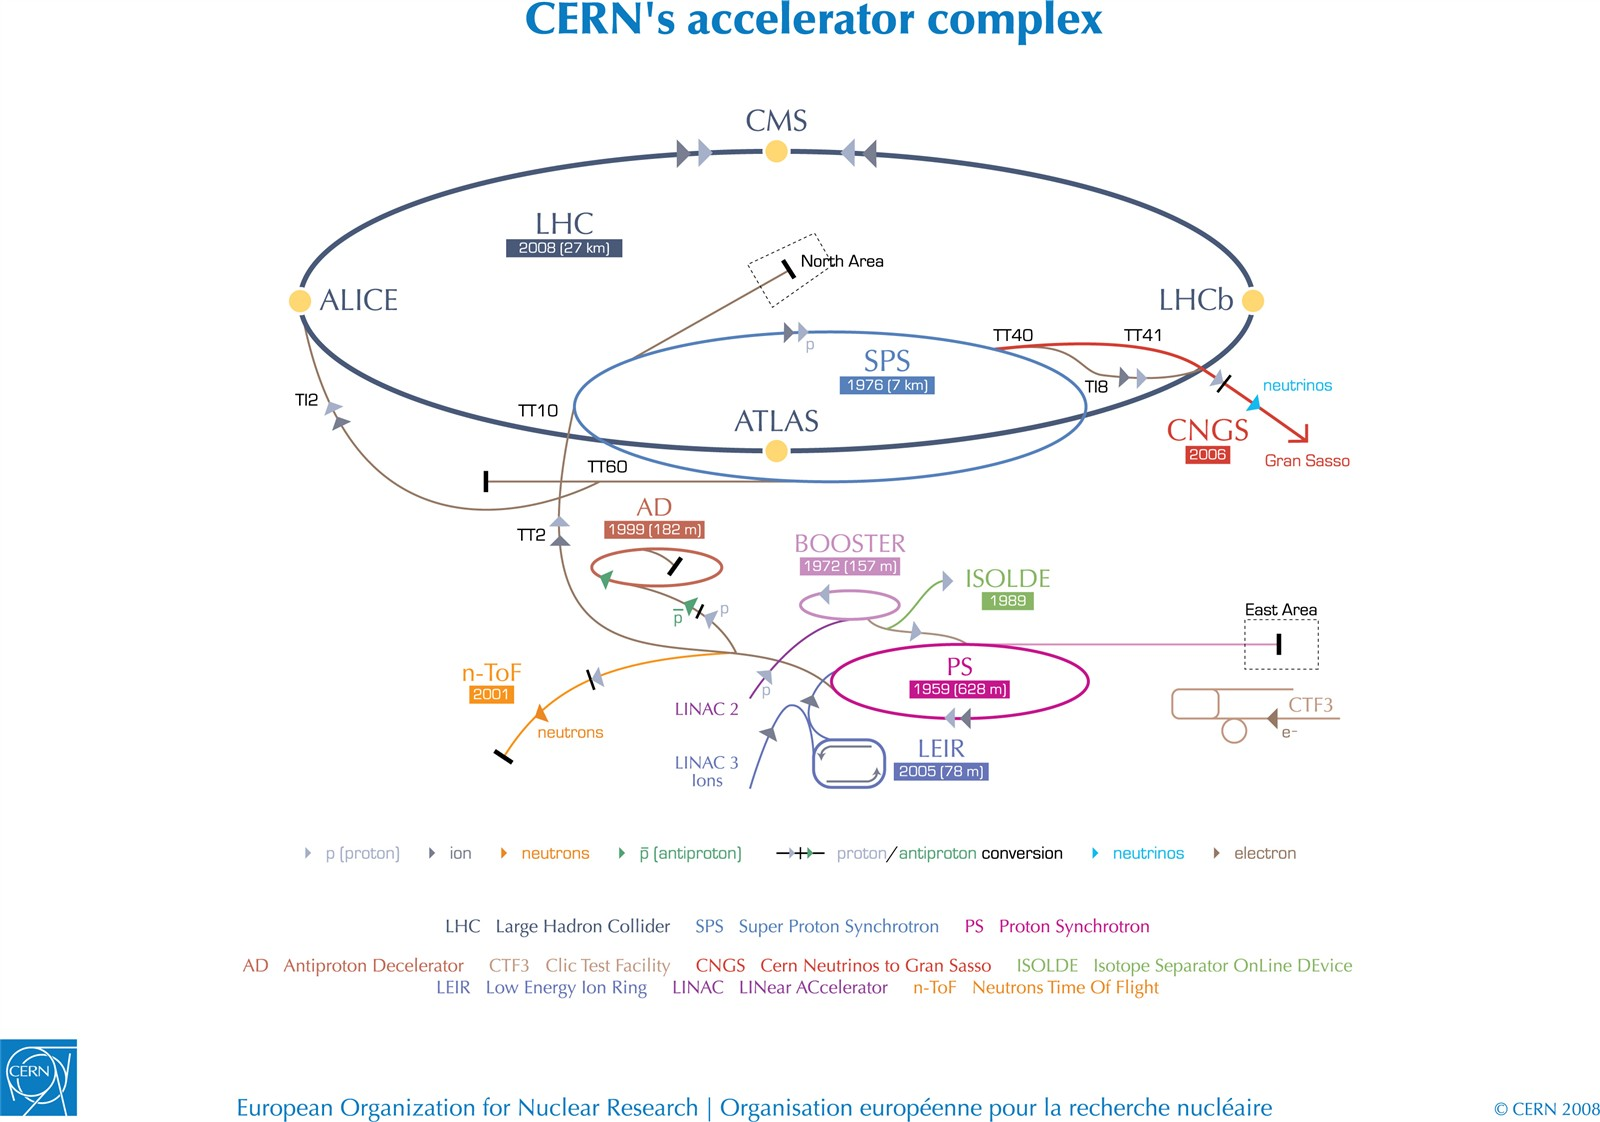
\includegraphics[width=0.95\textwidth]{Introduction/figures/cernaccelerators.jpg}
\end{center}
\label{fig:CERN-acc-complex}
\caption{The CERN accelerator complex, showing both the proton and heavy ion (lead) accelerator chains from LINACs 2 and 3 up to the LHC. Different experimental uses are highlighted in the diagram.}
\end{figure}

\begin{enumerate}
\item{Introduction to CERN}
\item{Introduction to the LHC}
\item{Luminousity - The Operational Figure of Merit}
\begin{itemize}
\item{Peak Luminousity - Equation and factors that control it}
\item{Integrated Luminousity - Up time and availability is important}
\end{itemize}
\item{Beam Dynamics}
\begin{itemize}
\item{Optics and Transverse Beam Dynamics}
\item{Longitudinal Dynamics - Energy change in a cavity}
\item{Chromaticity and Dispersion}
\end{itemize}
\end{enumerate}